\documentclass[17pt, t, lualatex]{beamer}



\title{Hidrodinámica del Río Magdalena a la altura de Barrancabermeja}
\date{\today}
\institute[UJTL]{Universidad Jorge Tadeo Lozano}
\author{Ludwig Alvarado Becerra}

\usepackage{amsmath, amssymb, mathtools}
\usepackage[spanish]{babel}
\usepackage{biblatex}
\usepackage{hyperref}
\usepackage{xurl}

\addbibresource{referencias.bib}  % Make sure your .bib file is correctly named


\addbibresource{referencias.bib}

% Probably load as late as possible
% Other options are
% - engine=pdflatex to compile in pdfLaTeX (with different fonts),
% - mathshape=rm to use serif font for math,
% - mathsahpe=custom to not set any math font (so that you can define your own math fonts)
\usetheme[engine=lualatex, mathshape=sf, fontdir=kthpq-files/fonts/Figtree/]{kthpq}
\setmonofont{Bitstream Vera Sans Mono}[Scale=.9]

% Custom colors (see beamercolorthemecustom.sty for more details)
% \usecolortheme{custom}

% Modify the headline template: KTH-full, KTH-section-only, or KTH-frametitle-only.
% \setbeamertemplate{headline}[KTH-full]

% Custom footline
% \setfootline{left}{center}{right}

\begin{document}

\inserttitlepage

\section{Exploración de datos}

\insertsectionpage

\begin{frame}[allowframebreaks]
  \frametitle{Exploración de datos}
  De acuerdo a Deaton\cite{deaton1999dynamic} la disponibilidad de los siguientes datos es crucial:

  \begin{itemize}
    \item Características topográficas del canal:
          \begin{itemize}
            \item Longitud.
            \item Elevación.
            \item Pendientes,
          \end{itemize}
    \item Características de transporte del canal:
          \begin{itemize}
            \item Elevación de la superficie del agua.
            \item Ancho.
            \item Coeficientes de rugosidad.
          \end{itemize}
    \item Datos de la condición final de frontera.
    \item Condición inicial.
  \end{itemize}

\end{frame}

\begin{frame}[allowframebreaks]
  \frametitle{Región de estudio}
  
  \begin{figure}[ht]
    \centering
    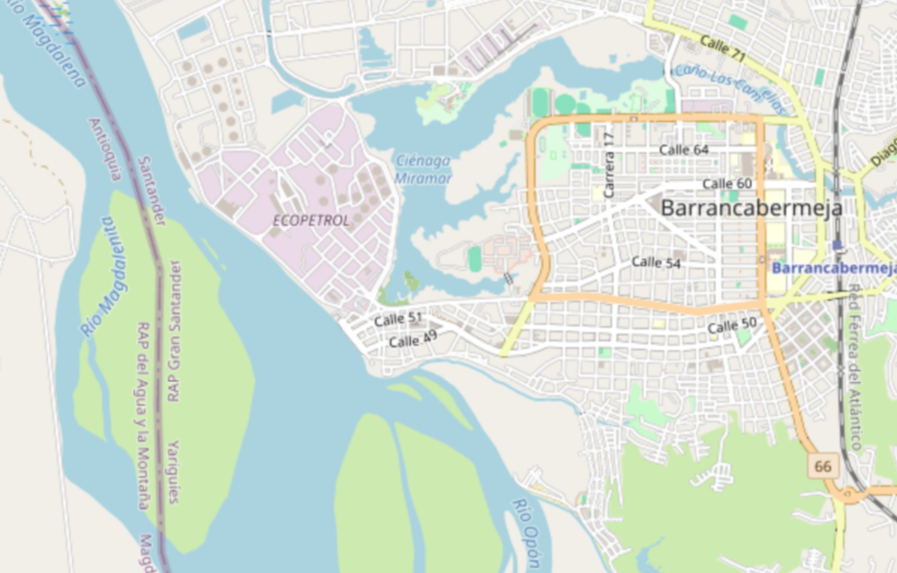
\includegraphics[width=0.5\textwidth]{img/OSM-1.png}
    \caption{Región a estudiar del Río Magdalena. Datos de \textit{OpenStreetMap} (OSM)\cite{openstreetmap_magdalena2025}}
  \end{figure}

  \begin{figure}[ht]
    \centering
    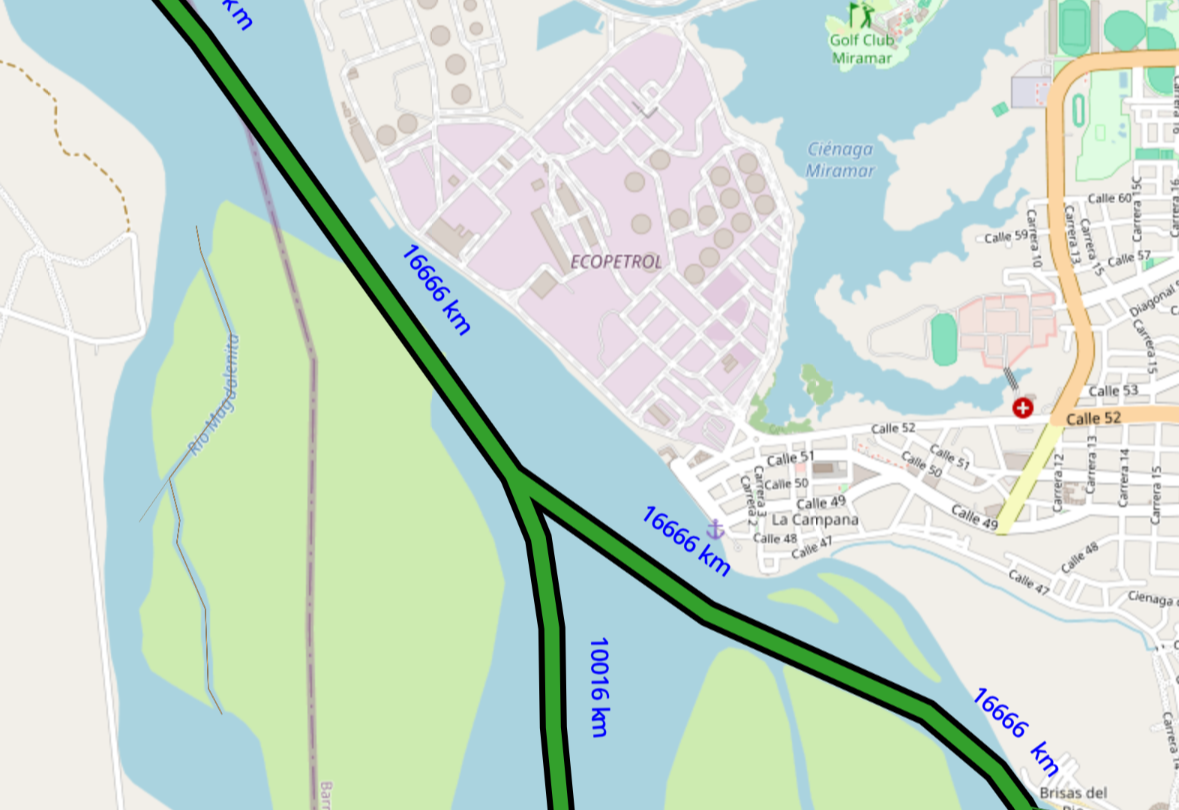
\includegraphics[width=0.5\textwidth]{img/Waterway.png}
    \caption{Río Magdalena. Datos sacados de \textit{Waterway}\cite{waterwaymap2025}}
  \end{figure}

  \begin{figure}[ht]
    \centering
    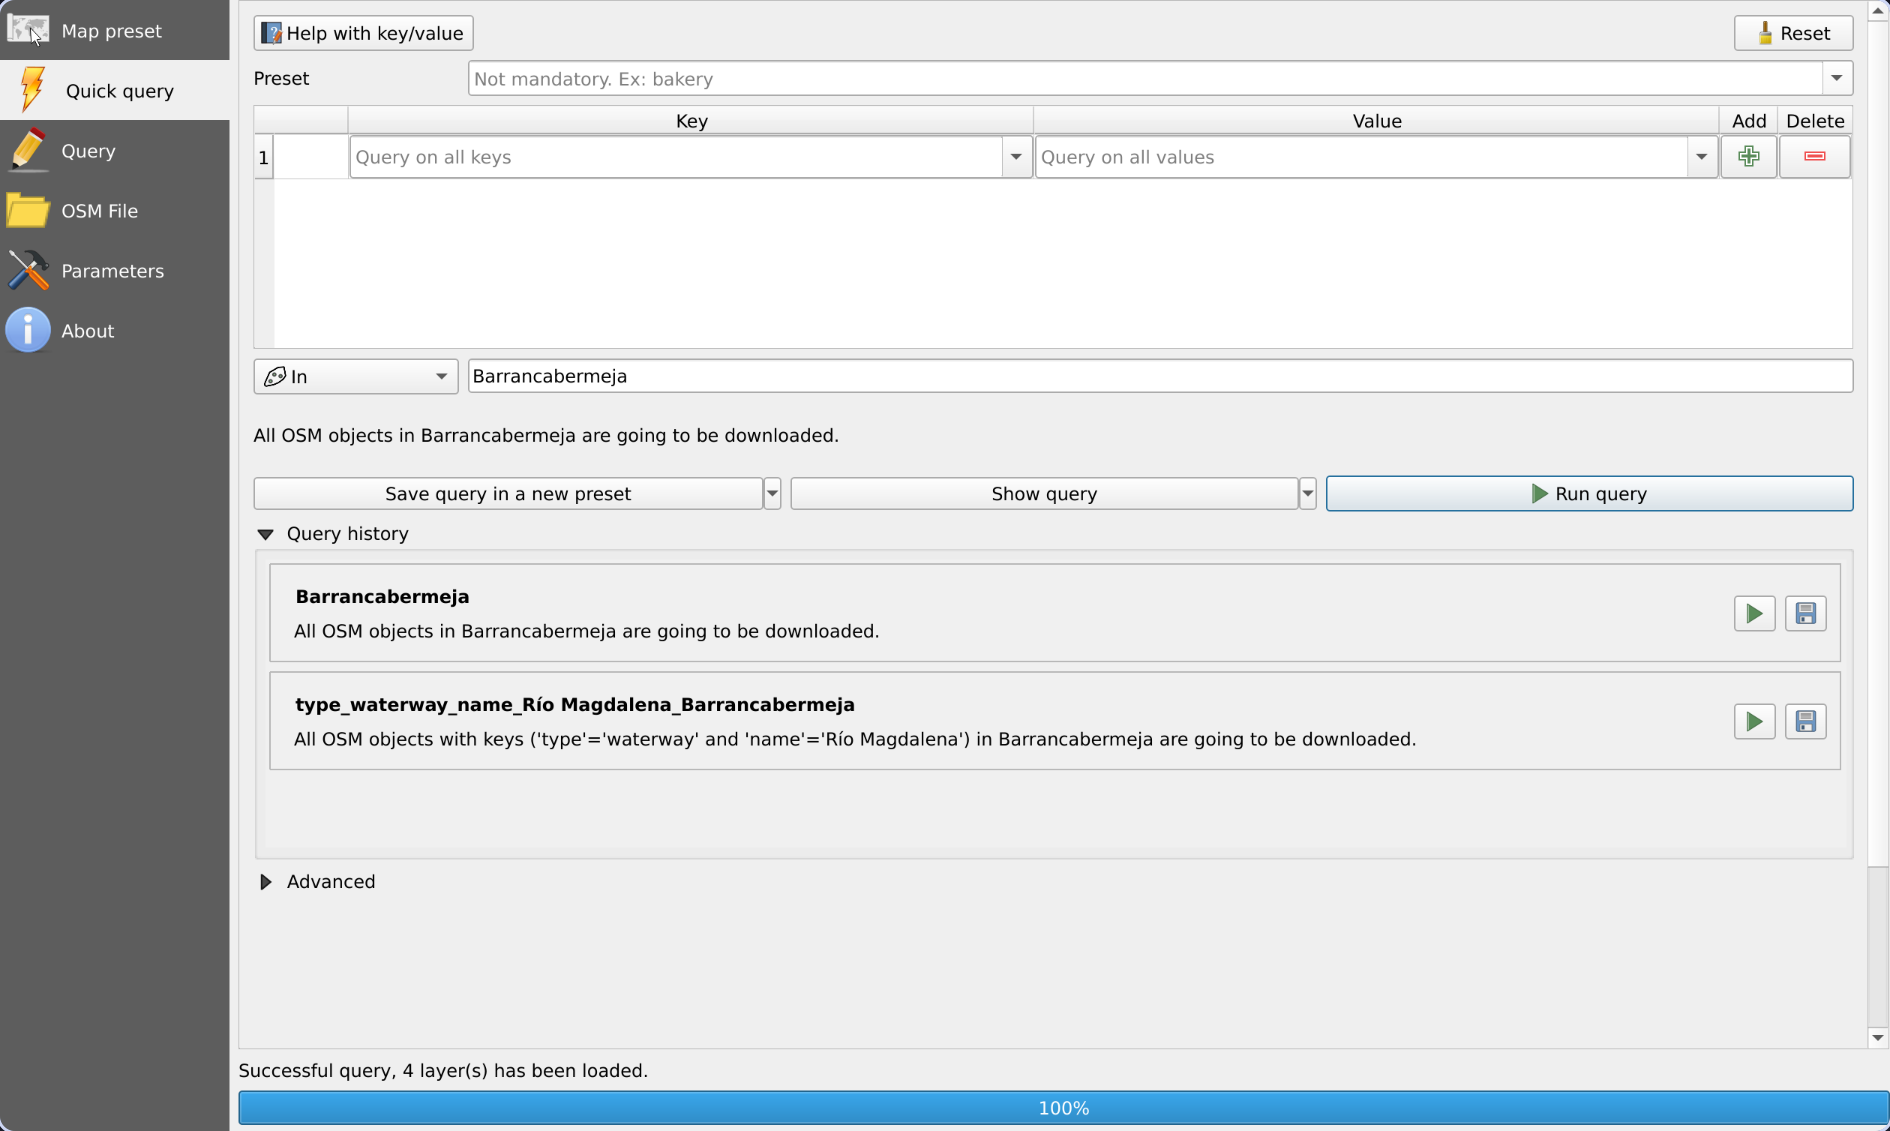
\includegraphics[width=0.5\textwidth]{img/QGIS-5.png}
    \caption{Consulta de datos utilizando QuickOSM\cite{quickosm2025}}
  \end{figure}


  \begin{figure}[ht]
    \centering
    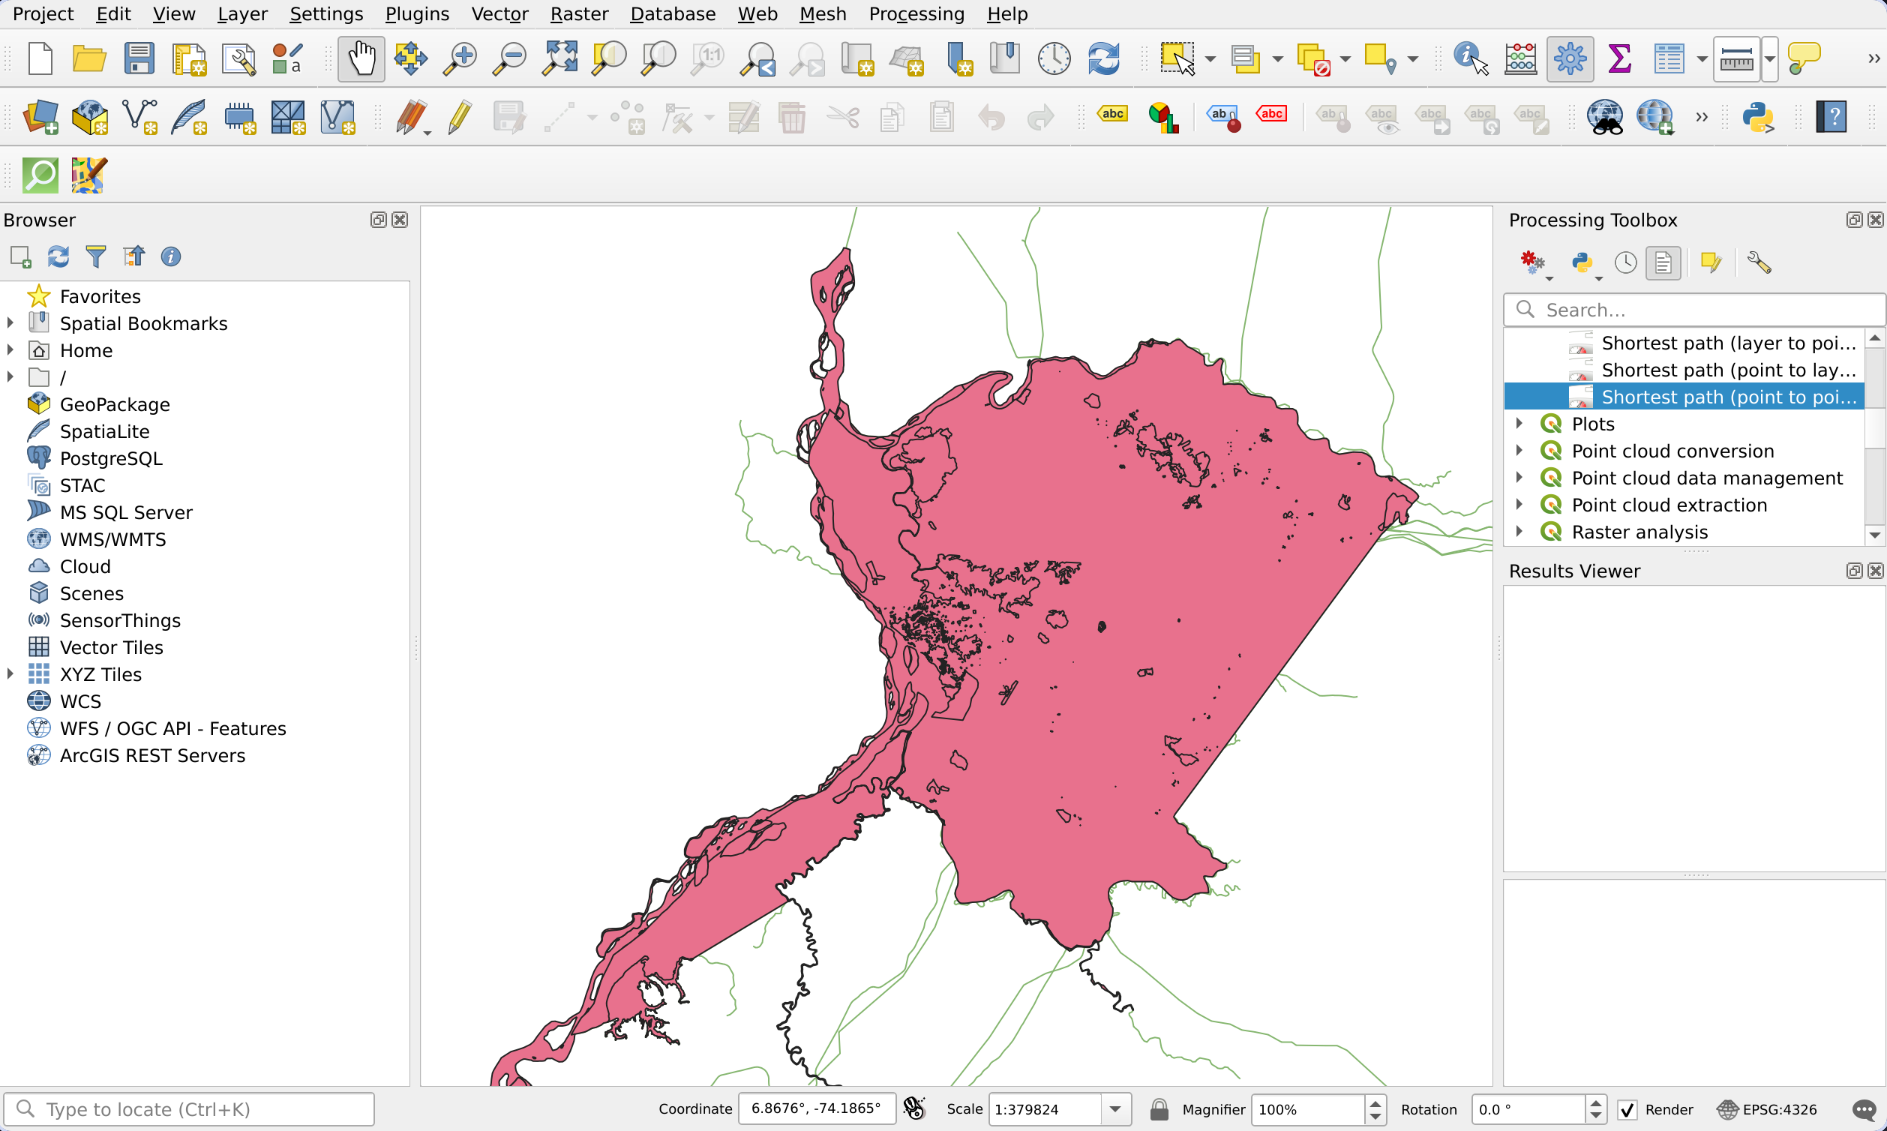
\includegraphics[width=0.55\textwidth]{img/QGIS-1.png}
    \caption{Región de Barrancabermeja, elaboración propia en QGIS\cite{qgis2025}, datos de OSM\cite{openstreetmap_magdalena2025}.}
  \end{figure}


  \begin{columns}
    \begin{column}{.3\textwidth}
      \begin{itemize}
        \item Se filtra la capa del Río Magdalena y se le cambia el color para que destaque.
      \end{itemize}
    \end{column}

    \begin{column}{.7\textwidth}
      \begin{figure}[ht]
        \centering
        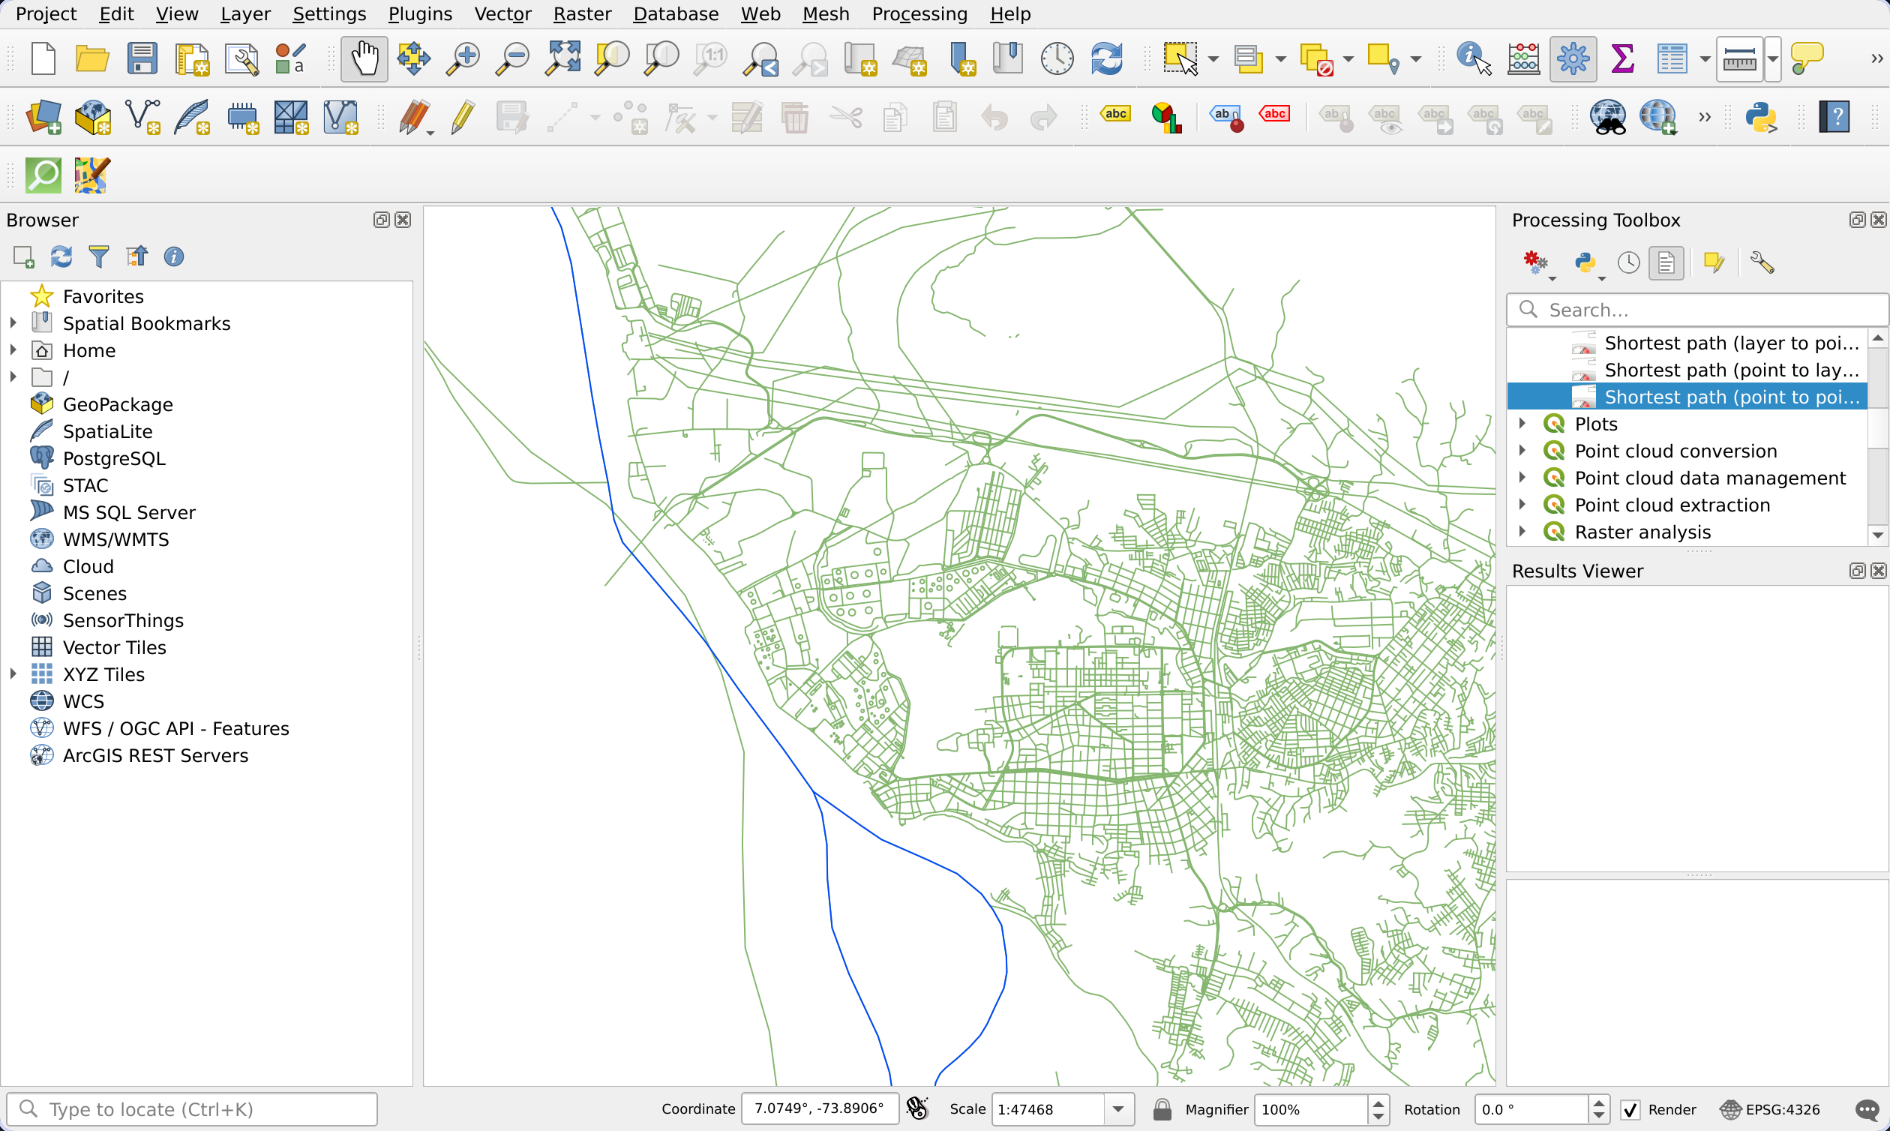
\includegraphics[width=0.8\textwidth]{img/QGIS-2.png}
        \caption{Elaboración propia.}
      \end{figure}
    \end{column}
  \end{columns}


  \begin{columns}
    \begin{column}{.3\textwidth}
      \begin{itemize}
        \item Utilizar \texttt{Vector} > \texttt{Geometry Tools} > \texttt{Extract Vertices...}
      \end{itemize}
    \end{column}

    \begin{column}{.7\textwidth}
      \begin{figure}[ht]
        \centering
        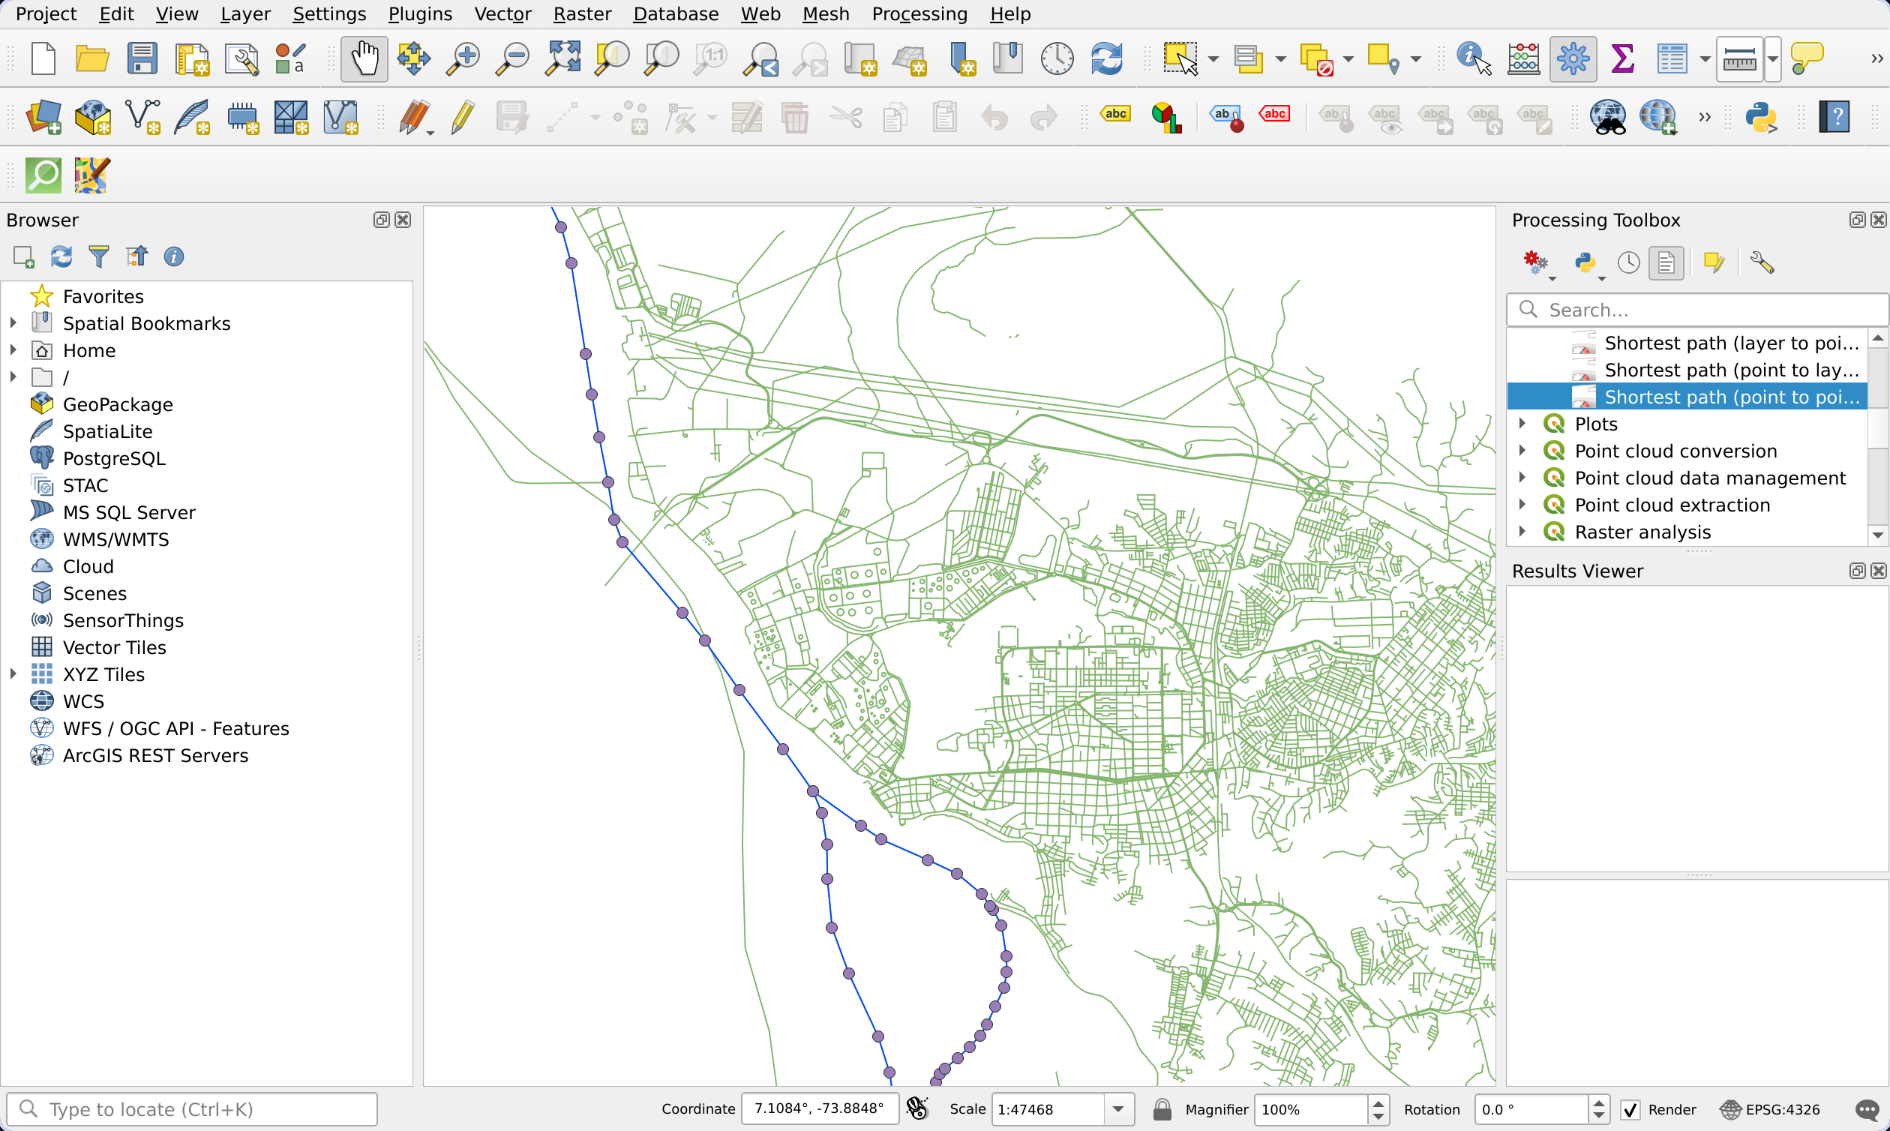
\includegraphics[width=0.8\textwidth]{img/QGIS-3.png}
        \caption{Elaboración propia.}
      \end{figure}
    \end{column}
  \end{columns}

  \begin{columns}
    \begin{column}{.3\textwidth}
      \begin{itemize}
        \item Se seleccionan el segmento que se de interés para el estudio. 
      \end{itemize}
    \end{column}

    \begin{column}{.7\textwidth}
      \begin{figure}[ht]
        \centering
        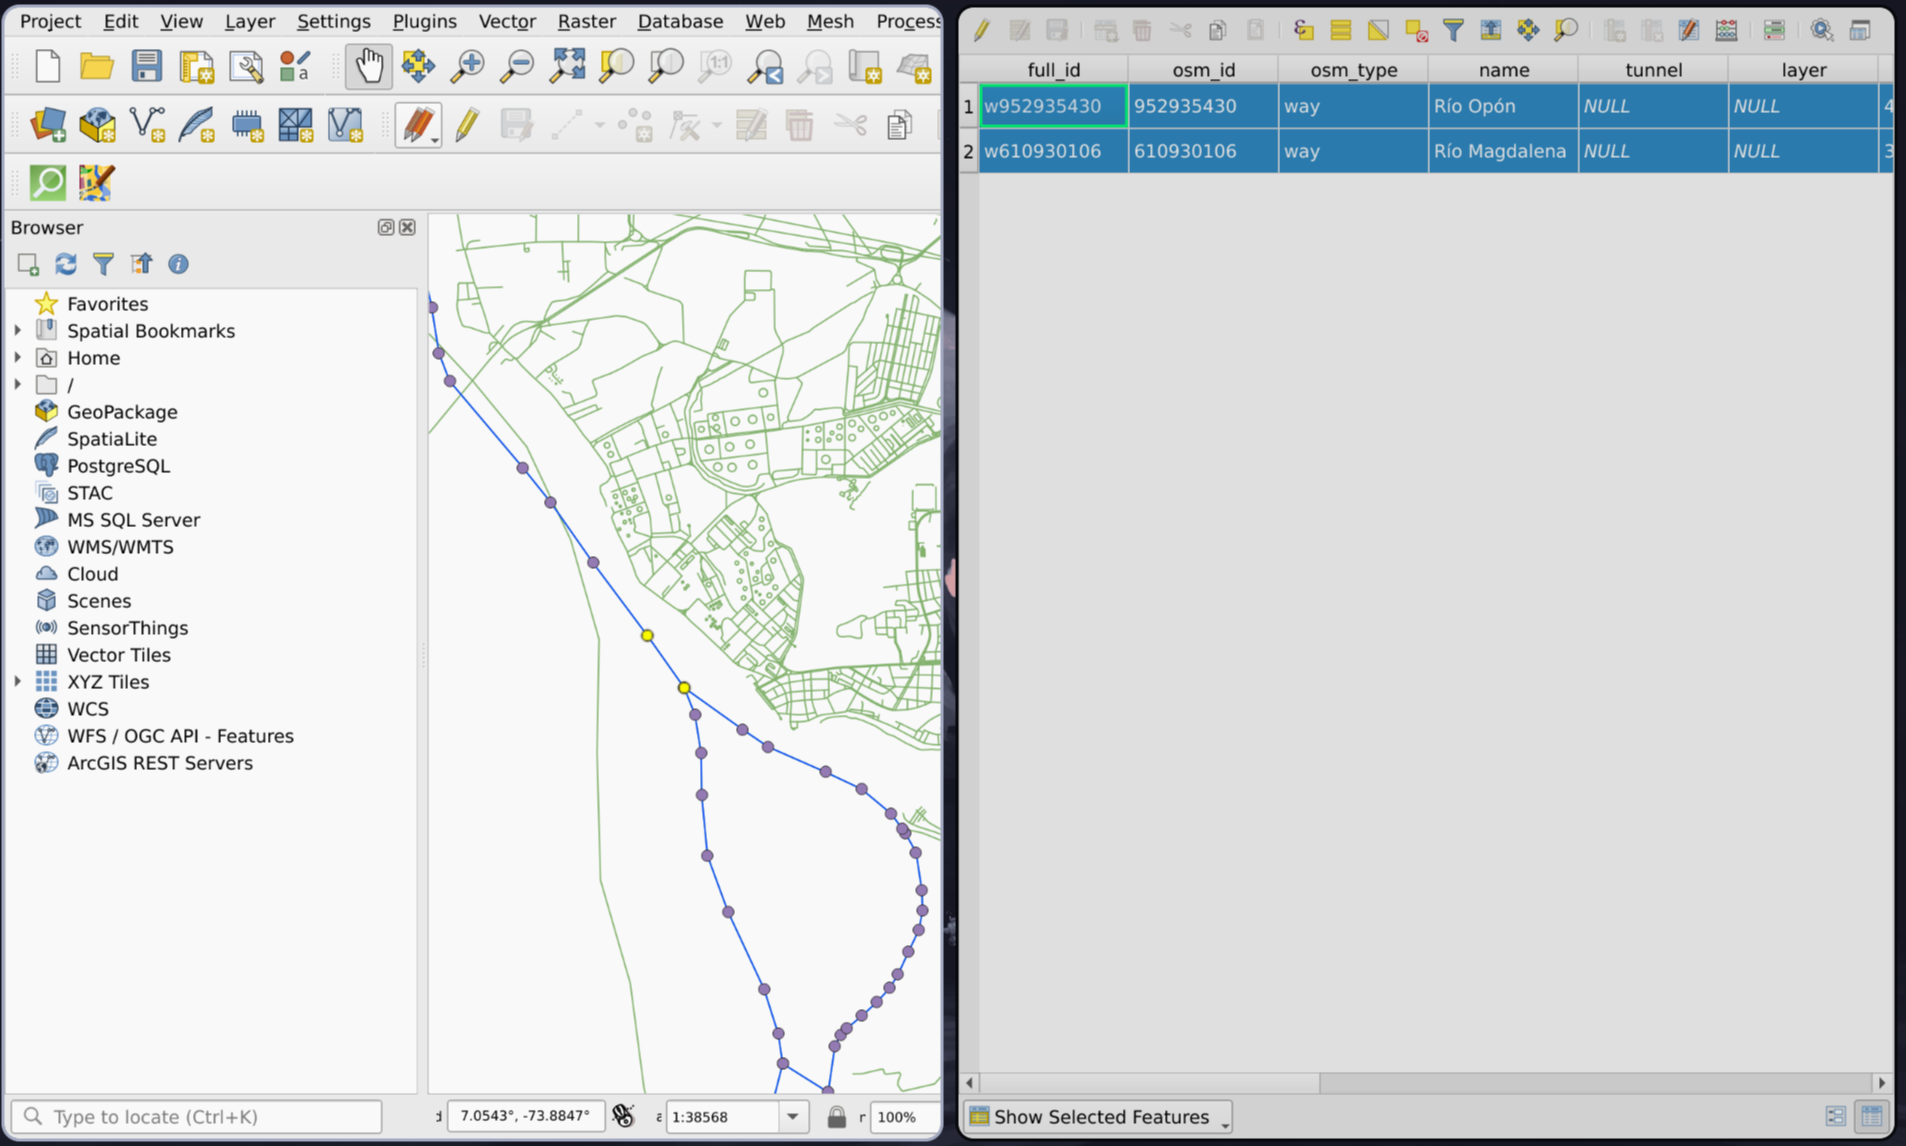
\includegraphics[width=0.8\textwidth]{img/QGIS-4.png}
        \caption{Elaboración propia.}
      \end{figure}
    \end{column}
  \end{columns}

  \begin{columns}
    \begin{column}{.3\textwidth}
      \begin{itemize}
        \item Utilizando la herramienta de \texttt{Distance matrix...} se obtienen $472.7434 \text{ metros}$ .
      \end{itemize}
    \end{column}

    \begin{column}{.7\textwidth}
      \begin{figure}[ht]
        \centering
        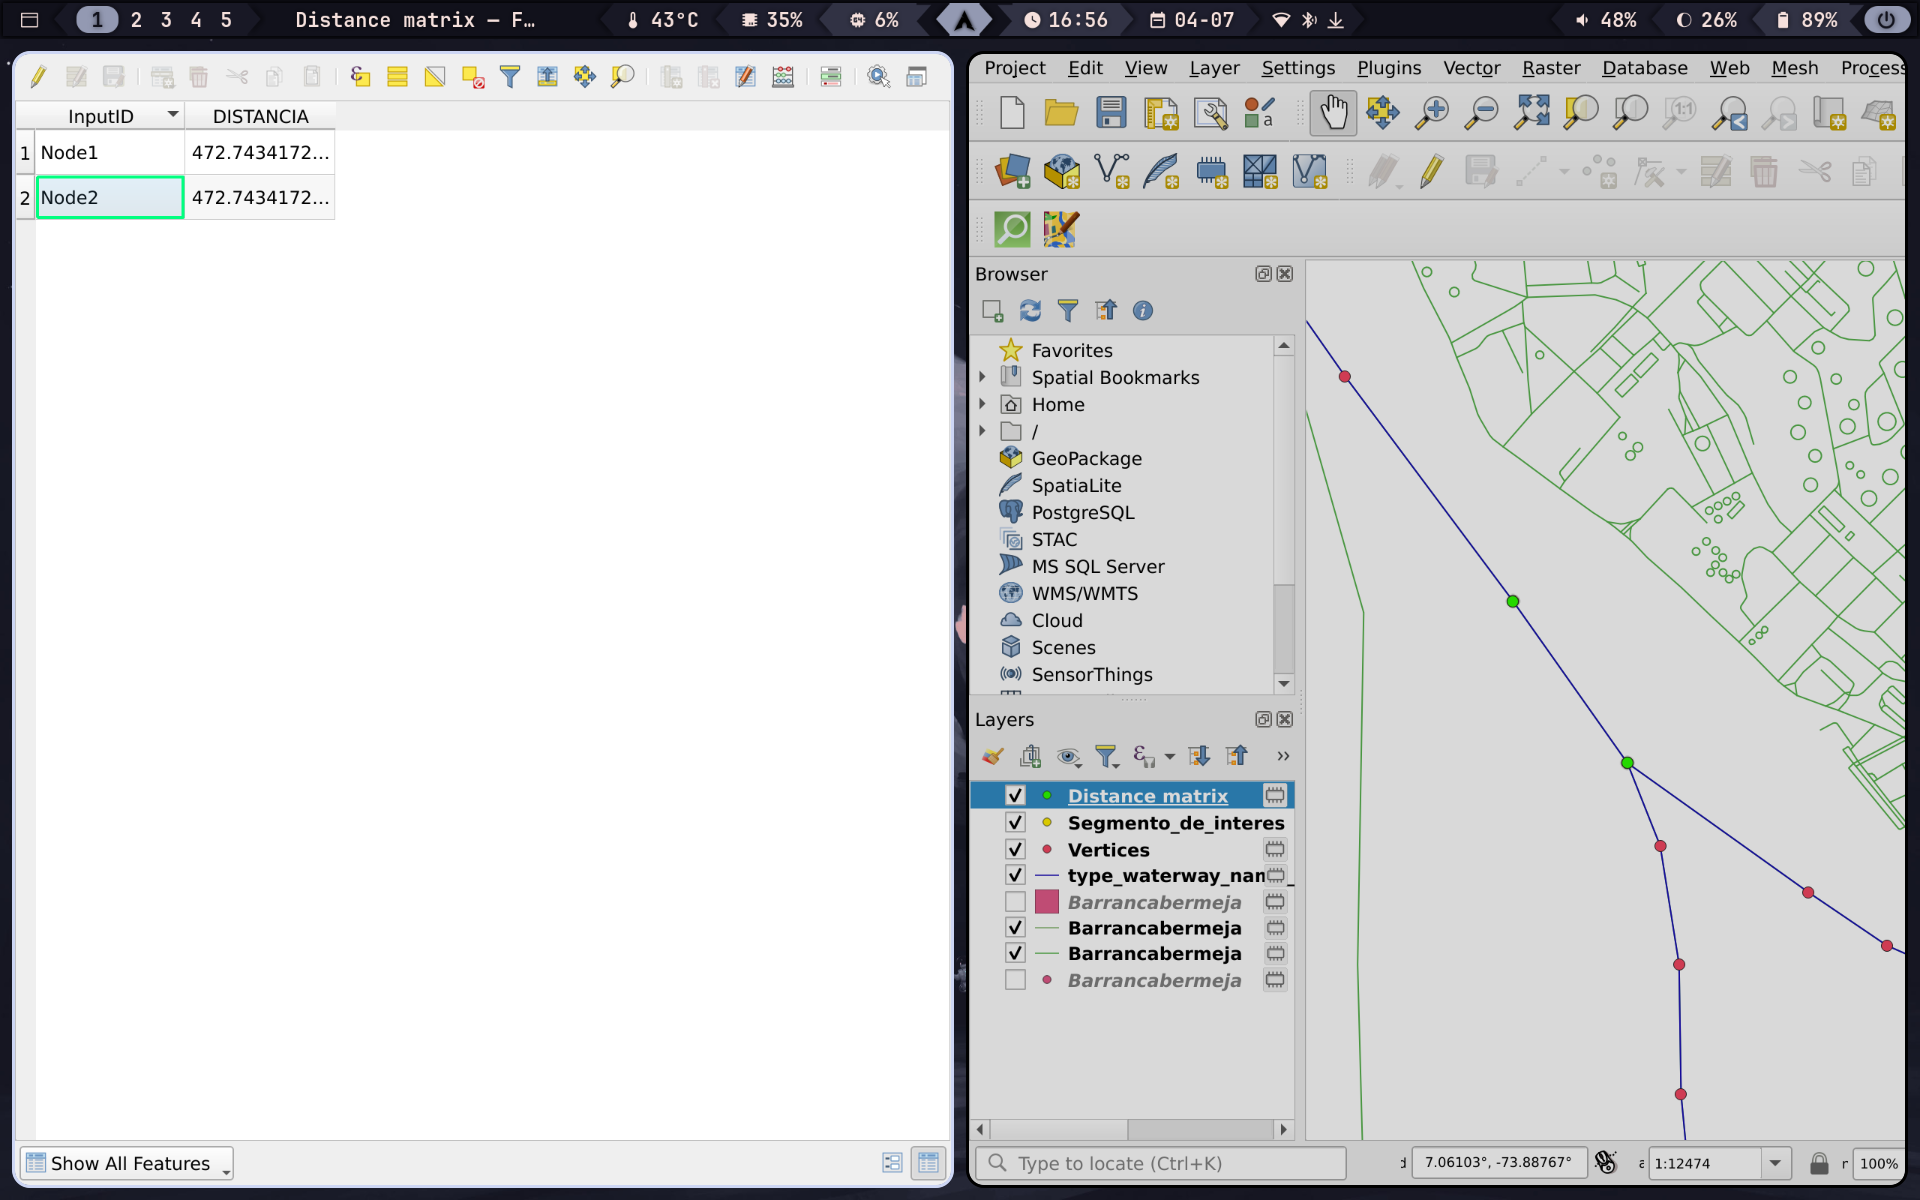
\includegraphics[width=0.7\textwidth]{img/QGIS-6.png}
        \caption{Elaboración propia.}
      \end{figure}
    \end{column}
  \end{columns}

\end{frame}

\begin{frame}
  \frametitle{Consulta del ancho}

  \begin{columns}
    \begin{column}{.3\textwidth}
      \begin{itemize}
        \item Usando la opción \texttt{Open Field Calculator} se puede consultar la información de estos datos como si fuera SQL.
        \item El resultado de esto son $300 \text{ metros}$
      \end{itemize}
    \end{column}

    \begin{column}{.7\textwidth}
      \begin{figure}[ht]
        \centering
        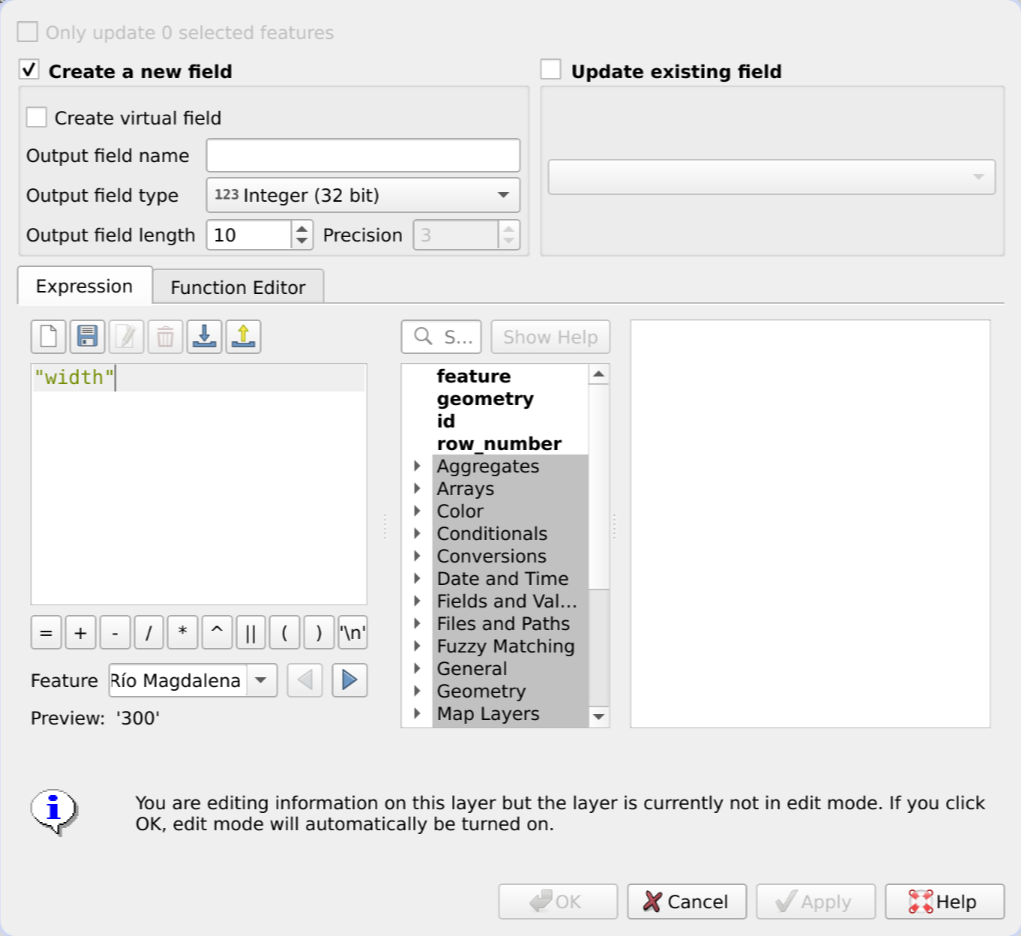
\includegraphics[width=0.5\textwidth]{img/QGIS-7.png}
        \caption{Consulta del ancho del Río Magdalena.}
      \end{figure}
    \end{column}
  \end{columns}



\end{frame}




\section{Referencias}

\insertsectionpage
\begin{frame}[allowframebreaks]{Referencias}
  \printbibliography
\end{frame}


\insertendpage

\end{document}
